Sobre una mesa lisa, de material aislante y en cada uno de los vértices de un cuadrado cuyos lados miden 10 cm, se encuentran fijas las cargas puntuales $Q_1$ = 5.0 $\mu$C, $Q_2$ = -5.0 $\mu$C y $Q_3$ = 5.0 $\mu$C, como se indica en la figura de este problema. En el vértice restante del cuadrado se deposita una pequeña esfera de masa $m$ = 100 g, electrizada con una carga $q$ = 2.0 $\mu$C. Determine la magnitud, la dirección y el sentido de la aceleración que adquirirá esta esfera.\\
(Constante eléctrica: $K = 9\times 10^{-9}$Nm$^2$/C$^2$)
\begin{figure}[h!]
  \centering
  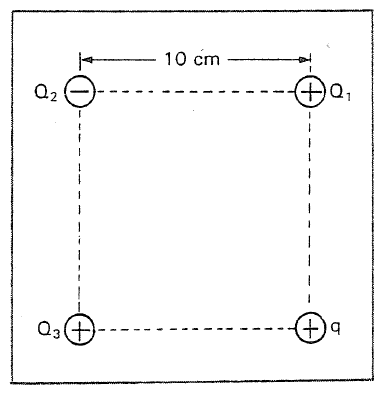
\includegraphics[scale=0.5]{figuras/fig_alvarenga_p825_19.png}
  \caption{Problema 21}
\end{figure}